
%%%%%%%%%%%%%%%%%%%%%%%%%%%%%%%%%%%%%%%%%%%%%%%%%%%%%%%%%%%%%%%%%%%%%%%%%%%%%%%%%%%%%%%%%%%%%%%%%
%
% Document:      DM  SST organisation chart reporting lines
%
% Based on the DM organisation chart reporting lines by William O'Mullane
%%%%%%%%%%%%%%%%%%%%%%%%%%%%%%%%%%%%%%%%%%%%%%%%%%%%%%%%%%%%%%%%%%%%%%%%%%%%%%

\documentclass{article}

\usepackage{times,layouts}
\usepackage{tikz,hyperref,amsmath}
\usetikzlibrary{positioning,arrows,shapes,decorations.shapes,shapes.arrows}
\usetikzlibrary{backgrounds,calc}

\usepackage[paperwidth=19cm,paperheight=13.0cm,
left=-2mm,top=3mm,bottom=0mm,right=0mm,
noheadfoot,marginparwidth=0pt,includemp=false ]{geometry}


\newcommand\showpage{%
\setlayoutscale{0.5}\setlabelfont{\tiny}\printheadingsfalse\printparametersfalse
\currentpage\pagedesign}


\hypersetup{pdftitle={DM SST organisation }, pdfsubject={Diagram illustrating the reporting lines in LSST SST DM Group},
pdfauthor={Leanne Guy}}


%%%%%%%%%%%%%%%%%%%%%%%%%%%%%%%%%%%%%%%%%%%%%%%%%%%%%%%%%%%%%%%%%%%%%%%%%%%%%%%%%%%%%%%%%%%%%%%%%
%
% Document:      Boxes and lines for all diagrams
%
%%%%%%%%%%%%%%%%%%%%%%%%%%%%%%%%%%%%%%%%%%%%%%%%%%%%%%%%%%%%%%%%%%%%%%%%%%%%%%

\tikzstyle{divbox}=[rectangle, rounded corners=3pt, draw=blue, top color=blue!30!white, bottom
color=white, very thick, minimum height=12mm, inner sep=3pt, text centered, text width=35mm]

\tikzstyle{arcbox}=[rectangle, rounded corners=3pt, draw=red, top color=yellow!50!white, bottom
color=white, very thick, minimum height=12mm, inner sep=2pt, text centered, text width=50mm]

\tikzstyle{psbox}=[rectangle, rounded corners=3pt, draw=red, top color=green!50!white, bottom
color=cyan, very thick, minimum height=10mm, inner sep=2pt, text centered, text width=35mm]

\tikzstyle{pobox}=[rectangle, rounded corners=3pt, draw=red, top color=blue!50!white, bottom
color=cyan, very thick, minimum height=10mm, inner sep=2pt, text centered, text width=35mm]

\tikzstyle{docbox}=[rectangle, rounded corners=3pt, draw=black, fill=cyan!50!white, 
 very thick, minimum height=12mm, inner sep=2pt,  text centered, text width=30mm]

\tikzstyle{docboxm}=[rectangle, rounded corners=3pt, draw=black, fill=red!50!white, 
 very thick, minimum height=12mm, inner sep=2pt,  text centered, text width=30mm]

\tikzstyle{docboxicd}=[rectangle, rounded corners=3pt, draw=black, fill=green!70!white, 
 very thick, minimum height=12mm, inner sep=2pt,  text centered, text width=30mm]

\tikzstyle{gbox}=[rectangle, rounded corners=3pt, draw=orange!80!black, top color=orange!30!white,
bottom color=white, very thick, minimum height=12mm, inner sep=5pt, text badly ragged, text width=40mm]

\tikzstyle{mbox}=[rectangle, rounded corners=3pt, draw=blue, top color=cyan!50!white, bottom
color=white, very thick, minimum height=8mm, inner sep=2pt, text centered, text width=30mm]

\tikzstyle{line}=[-, thick]
\tikzstyle{sline}=[-, thick, dashed, olive]
\tikzstyle{dline}=[->, thick, cyan]
\tikzstyle{tline}=[->, thick, dashed, blue]
\tikzstyle{pline}=[->, thick,  black!60!white]

\xdefinecolor{softviolet}{rgb}{0.85, 0.8, 1.0}




\begin{document}

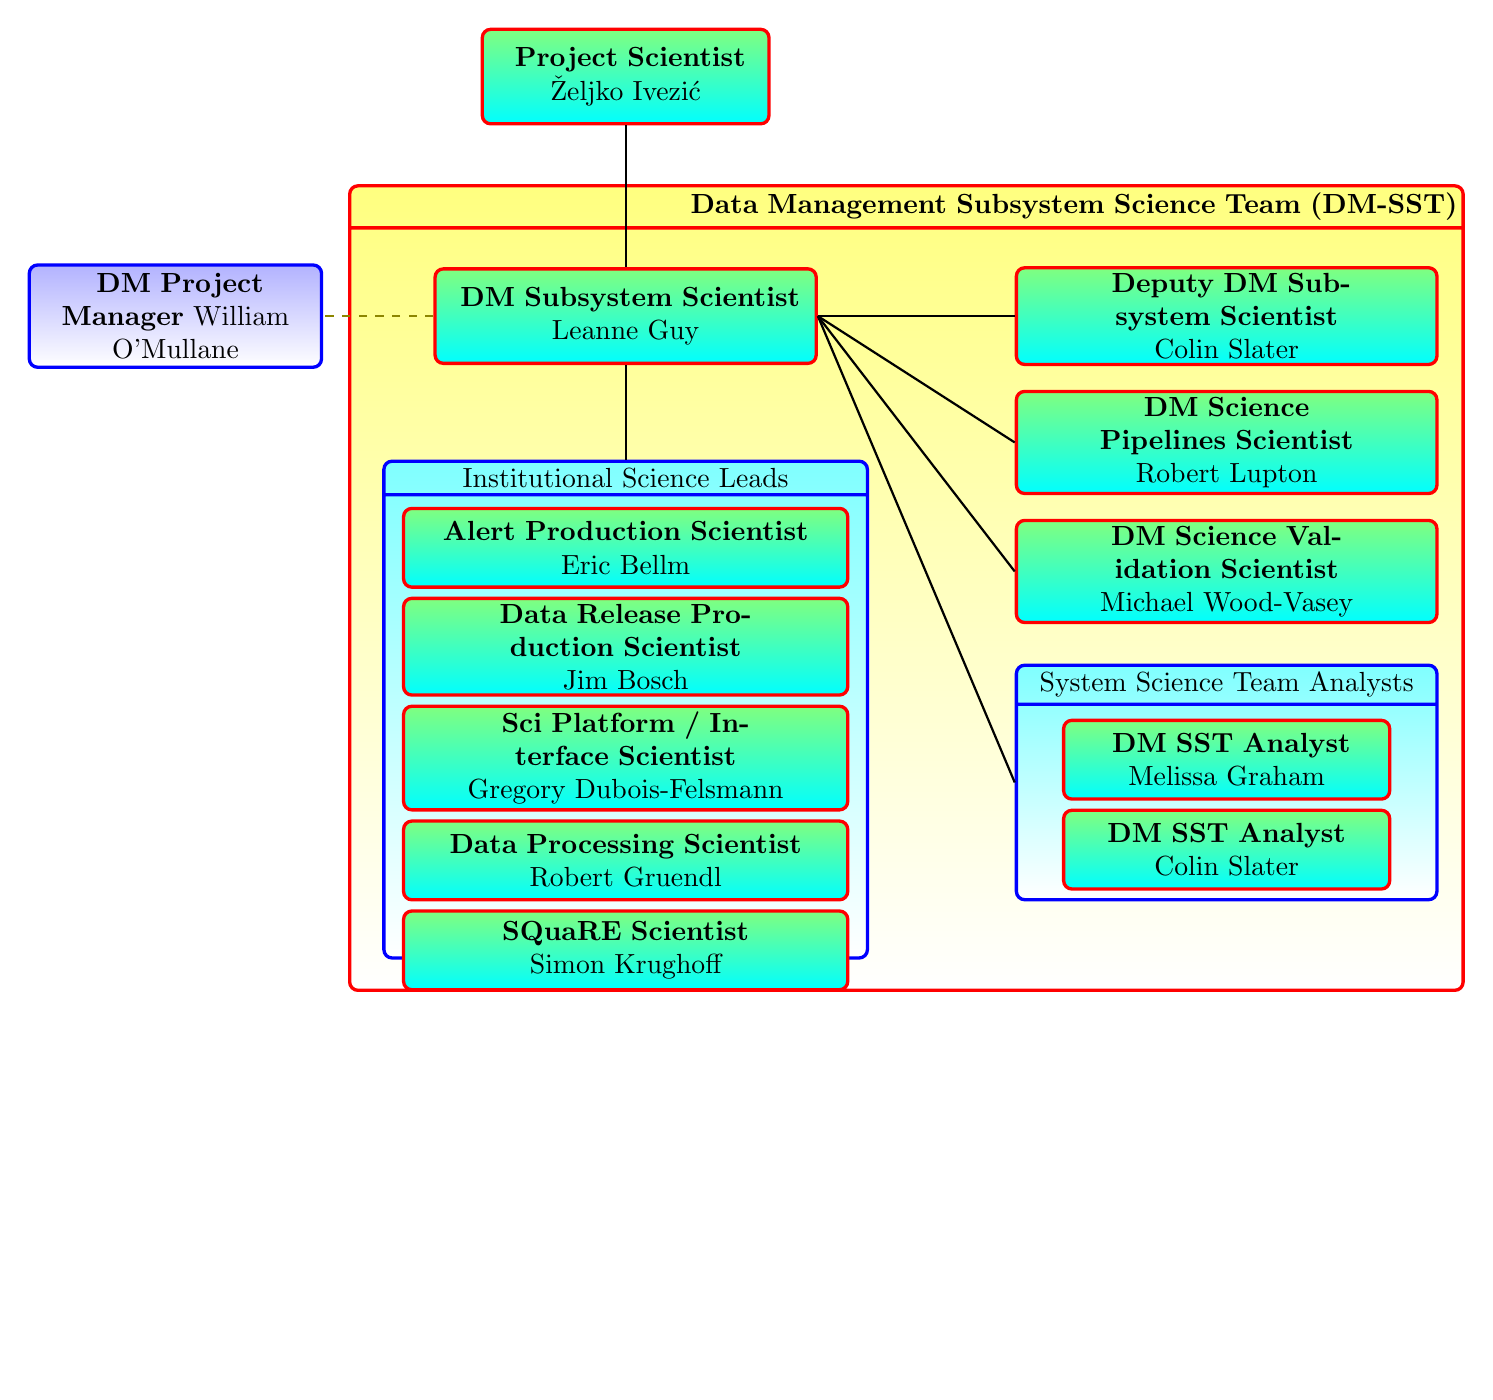
\begin{tikzpicture}[node distance=0mm]


    \node (dm) [arcbox, align=right, text width=14cm,  minimum height=10mm, rectangle split, rectangle split parts=2]
    { \hspace{0.1cm} \textbf{Data Management Subsystem Science Team (DM-SST)}
	   \nodepart{second} \vspace{95mm}
	};

    \node (dmpsanc) [above=-1.8 of dm.north]{};
    \node (dmps) [psbox, left=1.0cm of dmpsanc, minimum height=12mm, text width=47mm] {\textbf{ DM Subsystem Scientist}\\ Leanne Guy };
    \node (ddmps) [psbox, right=2.5cm of dmps, minimum height=12mm, text width=52mm] {\textbf{ Deputy DM Subsystem Scientist}\\ Colin Slater };
    \node (ps) [psbox, above=1.8cm of dmps, minimum height=12mm] {\textbf{  Project Scientist}\\ \v{Z}eljko Ivezi\'c};
    \node (dmpm) [divbox, left=1.4cm of dmps] {\textbf{ DM Project Manager} William O'Mullane};

    \node (udmpm) [below=49mm of dmpm, text width=0mm]{};
    \node (udmpm1) [below=24mm of dmpm, text width=0mm]{};
    \node (udmpm2) [below=125mm of dmpm, text width=0mm]{};

% Pipelines scientist
    \node (pipesci) [psbox, below =3mm of ddmps, text width=52mm, minimum height=12mm] {\textbf{DM Science Pipelines Scientist}\\ Robert Lupton};

% Verification Scientist
    \node (valsci) [psbox, below=3mm of pipesci, text width=52mm, minimum height=12mm] {\textbf{DM Science Validation Scientist}\\ Michael Wood-Vasey};

% InstLeads
            \node (instleads) [mbox, text width=60mm, rectangle split, rectangle split parts=2,  below=12mm of dmps]
                {
               Institutional Science Leads
                \nodepart{second} \vspace{57mm}
                };
    \node (apsc) [psbox, below=6mm of instleads.north, text width=55mm] {\textbf{Alert Production Scientist}\\ Eric Bellm };
    \node (drpsc) [psbox, below=1mm of apsc, text width=55mm] {\textbf{Data Release Production Scientist}\\ Jim Bosch};
    \node (suitsc) [psbox, below=1mm of drpsc, text width=55mm] {\textbf{Sci Platform / Interface Scientist}\\ Gregory Dubois-Felsmann};
    \node (dpsc) [psbox, below=1mm of suitsc, text width=55mm] {\textbf{Data Processing Scientist}\\ Robert Gruendl};
    \node (sqsc) [psbox, below=1mm of dpsc, text width=55mm] {\textbf{SQuaRE Scientist}\\ Simon Krughoff  };


%SST  analysts
            \node (sstanal) [mbox, text width=52mm, rectangle split, rectangle split parts=2, below=0.5cm of valsci.south ]
                {
                System Science Team Analysts
                \nodepart{second} \vspace{23mm}
                };
    \node (sstanal-mlg) [psbox, below=7mm of sstanal.north, text width=40mm] {\textbf{ DM SST Analyst }\\ Melissa Graham };
    \node (sstanal-cts) [psbox, below=1mm of sstanal-mlg, text width=40mm] {\textbf{DM SST Analyst}\\ Colin Slater};

   
%%% Legend 
%\node (leg) [lbox, below=4cm of admin, text width=35mm,  minimum height=10mm, rectangle split, rectangle split parts=2]
%    { \hspace{0.1cm} \textbf{Legend}
%           \nodepart{second} \vspace{30mm}
%        };
 %\node(snode) [psbox,below=0.7cm of leg.north, text width=30mm] {Science Role};
 %\node(pnode) [mbox,below=0.1cm of snode, text width=30mm] {Technical Role};
 %\node(mnode) [mbox,below=0.1cm of pnode, text width=30mm] {Managment/other Role};

   \draw[line] (dmps.north) --  (ps.south);
    \draw[sline] (dmps.west) --  (dmpm.east);
   \draw[line] (ddmps.west) --  (dmps.east);
   
    \draw[line] (dmps.east) --  (pipesci.west);
     \draw[line] (dmps.east) --  (valsci.west);
     \draw[line] (dmps.south) --  (instleads.north);
    \draw[line] (dmps.east) --  (sstanal.west);
      
\end{tikzpicture}
\end{document}
